\chapter{Sensors} 
\label{sensors}

The {\bf Sensors} in this report refer to the separate sensors connected to the body of the patient which collects raw measurements of vital sign paramaters, conditions the data so that it is suitable for analogue to digital conversion, and converts the data into a digital signal that can be interpreted by the platform ({\bf Terminals}). \\

The sensors used in this project are enumerated as follows with the respective vital sign parameter measured: 

\begin{enumerate}
	\item ECG - AD8232 Heart Rate Monitor 
	\item PPG - 
	\item EEG - 
	\item Blood Pressure - 
	\item Blood Temperature - Thermistor coupled with Phase Shift Oscillator
\end{enumerate}

The following sections below further discusses the reason behind the choices made for the individual sensors, the mechanism of operation, and how it interfaces with the entire system. 

\section{ECG}

The ECG front end design consists of a number of parts. 

The typical range of an ECG signal lies between $0.01\sim 300Hz$ and $0.05\sim 3mV$ in terms of frequency and amplitude respectively \cite{nisignalamplitude}. The voltages sampled from the surface of the skin through electrodes are too miniscule to be directly plotted and displayed. In addition, there are multiple frequencies which are of interest in ECG signals but the raw measurements will contain unwanted signal artifacts from other sources. Hence, it is necessary to amplify and filter the signal before any analysis or visualisation is performed.  

In 1997, Strohmenger \cite{strohmenger1997analysis} did an analysis of ventricular fibrillation ECG signal amplitude and frequency parameters for both successful and unsuccesful cardiac arrest countershocks. In this paper, the frequency range and amplitude range of both cases corroborates with the typical values stated above.  



\subsection{AD8232 IC ECG Sensor}

In this project, in line with the aim of producing a system that is a working proof of concept, a simplified version of the ECG is used. The AD8232 IC from Analog Digital was used \cite{ad8232datasheet}. 

\subsubsection{Front End}

The Analog Devices AD8232 was used to implement the ECG part of this project. The AD8232 is "an integrated signal conditioning block for ECG", "designed to extract, amplify, and filter small biopotential signals" \cite{ad8232datasheet}. The functional block diagram is included below in Figure \ref{ad8232functional}. 

\begin{figure}[H]
	\centering
	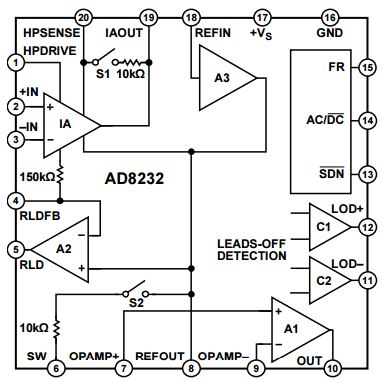
\includegraphics[width=0.5\linewidth]{ad8232funcdiagram.jpg}
	\caption{AD8232 Functional Block Diagram \cite{ad8232datasheet}}
	\label{ad8232functional}
\end{figure}

\begin{figure}[H]
	\centering
	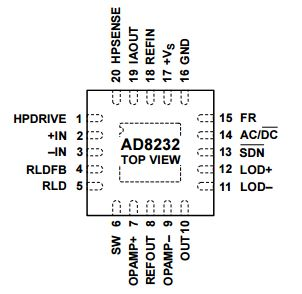
\includegraphics[width=0.4\linewidth]{ad8232pin.jpg}
	\caption{AD8232 Pin Configuration \cite{ad8232datasheet}}
	\label{ad8232pin}
\end{figure}

\subsubsection*{Theory of Operation of the AD8232}

\begin{figure}[H]
	\centering
	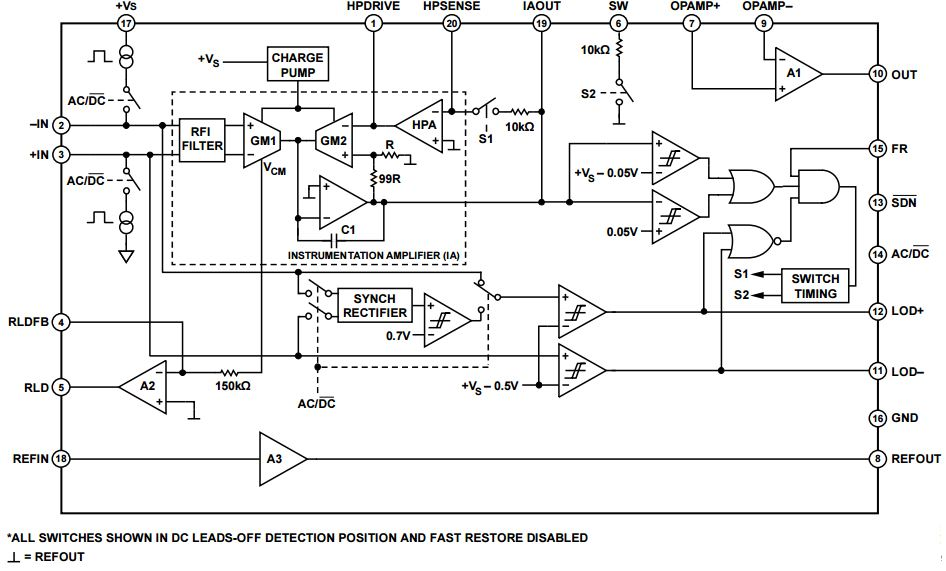
\includegraphics[width=\linewidth]{ad8232schematic.jpg}
	\caption{AD8232 Simplified Schematic Diagram \cite{ad8232datasheet}}
	\label{ad8232schematic}
\end{figure}

Figure \ref{ad8232schematic} above shows the architectural overview of the AD8232 chip from Analog Devices used for the "front end signal conditioning of cardiac biopotentials" \cite{ad8232datasheet} and is comprised of the following components: 

\begin{itemize}
	\item Specialized instrumentation amplifier (IA) - Amplifies ECG signals 
	\item Operational amplifier (A1) - For low pass filtering and supplying extra gain 
	\item Right leg drive amplifier (A2) - Improves common-mode signal rejection by inverting the signal 
	\item Midsupply reference buffer (A3) - Provides a reference signal for the IA by creating a virtual ground between the supply voltage and system ground 
	\item Leads off detection circuitry - Senses and indicates if the electrodes have been disconnected
	\item Automatic fast restore circuit - Decrease settling time of the ECG signal for a quicker response 
\end{itemize} 

\cite{ad8232analogdevices}

\cite{ad8232evalzuserguide}

\cite{ad8232datasheet}

\subsubsection*{AD8232 IC Cardiac Monitor Circuit Configuration}

The datasheet for the AD8232 provided by Analog Devices supplies a typical circuit setup and configuration for a cardiac monitoring as seen in the schematic diagram in Figure \ref{ad8232cardiacconfig} below \cite{ad8232datasheet}. A printed circuit board with this configuration could have been assembled and constructed using Altium Designer but due to time and cost constraints, an exact implementation of this circuit (with additional headers, an LED indicator, and a 3.5mm jack for biomedical pad connection) from SparkFun Electronics was used instead \cite{ad8232}.   

\begin{figure}[H]
	\centering
	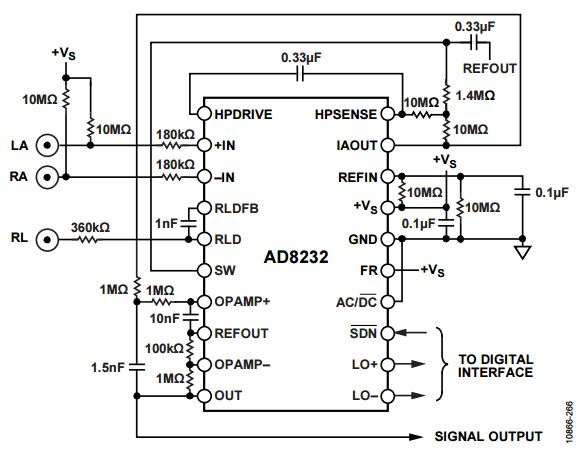
\includegraphics[width=0.7\linewidth]{ad8232cardiacconfig.jpg}
	\caption{Circuit Configuration for ECG Waveform Monitoring using the AD8232 \cite{ad8232datasheet}}
	\label{ad8232cardiacconfig}
\end{figure}
 
The schematic of the actual schematic capture of the AD8232 by SparkFun can be found in Appendix \ref{ad8232sfschematic}. The AD8232 Heart Monitor in Figure \ref{ad8232sfboard} is essentially a breakout board for the AD8232 integrated circuit provided by Analog Devices. 

\begin{figure}[H]
	\centering
	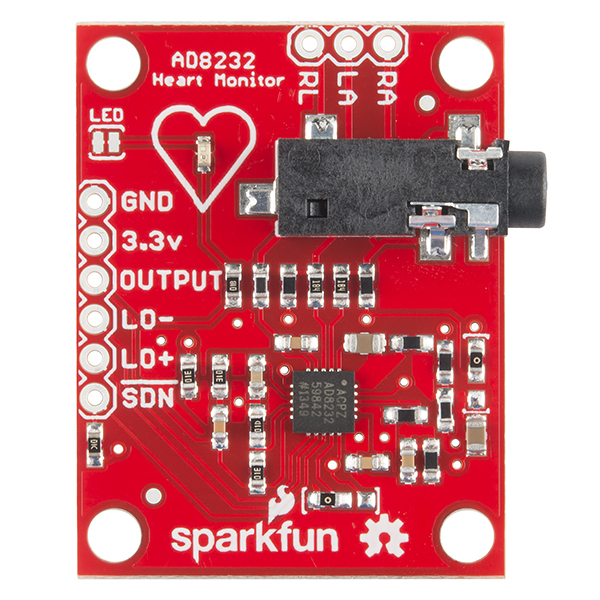
\includegraphics[width=0.4\linewidth]{ad8232sfboard.jpg}
	\caption{AD8232 Heart Rate Monitor from SparkFun Electronics \cite{ad8232}}
	\label{ad8232sfboard}
\end{figure}

CONSIDER PUTTING ALTIUM DESIGNER DESIGN

\subsubsection*{Complete AD8232 ECG Sensor Setup}

Due to the absence of an analog-to-digital converter, it is necessary to use a microcontroller which is capable of this conversion and serial communication through a USB port for prototyping. As such, an Arduino Pro Mini 328 (3.3V/8MHz) was used in the development of the interface. The design of the system was sourced from SparkFun Electronics \cite{ad8232}. 

The assembly of the complete AD8232 ECG sensor requires the following components \cite{ad8232}:

\begin{enumerate}
	\item Arduino Pro Mini 328 - 3.3V/8MHz (DEV-11114)
	\item SparkFun USB Mini-B Cable - 6 foot (CAB-11301)
	\item SparkFun FTDI Basic Breakout - 3.3V (DEV-09873)
	\item Break Away Headers - Straight (PRT-00116)
	\item Sensor Cable - Electrode Pads (3 connector) (CAB-12970)
	\item Biomedical Sensor Pad (10 pack) (SEN-12969) 
	\item SparkFun Single Lead Heart Rate Monitor - AD8232 (SEN-12650) 
\end{enumerate}

These components are assembled in the pattern found in Figure \ref{ad8232sffritzing}. 

\begin{figure}[H]
	\centering
	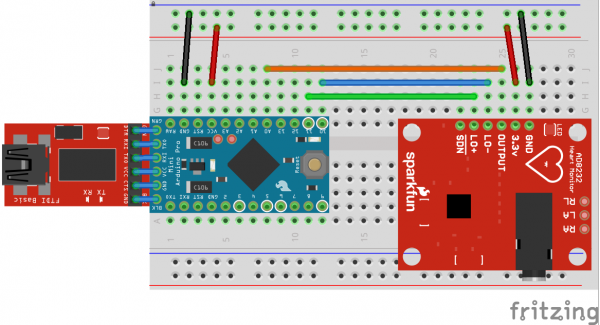
\includegraphics[width=0.9\linewidth]{ad8232fritzing.png}
	\caption{AD8232 Connection Diagram using Fritzing \cite{ad8232}}
	\label{ad8232sffritzing}
\end{figure}

In terms of the pin connections between the AD8232 and the Arduino Pro Mini, the connections are found in Table \ref{ad8232pinconfigurationtable}.

\begin{table}[H]
	\centering
	\caption{Pin Configuration for the AD8232 and the Arduino Pro Mini \cite{ad8232}}
	\label{ad8232pinconfigurationtable}
	\begin{tabular}{|l|l|l|}
		\hline
		\textbf{Board Label} & \textbf{Pin Function} & \textbf{Arduino Connection} \\ \hline
		GND                  & Ground                & GND                         \\ \hline
		3.3v                 & 3.3v Power Supply     & 3.3v                        \\ \hline
		OUTPUT               & Output Signal         & A0                          \\ \hline
		LO-                  & Leads-off Detect -    & 11                          \\ \hline
		LO+                  & Leads-off Detect +    & 10                          \\ \hline
		SDN                  & Shutdown              & Not used                    \\ \hline
	\end{tabular}
\end{table}


The complete circuit can be found in the Figure below 

FIGUREEEEEEEEEEEEEEEEEEEEEEEEEEEEEEEEEEEEEEEE

To circumvent the need of using a breadboard, a PCB shield for the AD8232 and the Arduino Pro Mini was designed to accomodate both breakout boards on a single board without the need for wires to connect the internal components. The PCB design can be found in Appendix \ref{ecgshieldpcb}. 

- Uploaded and compiled sample Arduino code from SparkFun GitHub repository. 
- Need to change board type to Arduino Pro Mini 328 - 3.3V/8MHz. 



\section{Blood Temperature}

\subsection{Thermistor}

One of the methods to measure body temperature is through measuring heat conduction via direct physical contact with the patient's body. As a thermistor is a temperature-dependent resistor, the resistance of a thermistor varies with temperature. The property of thermistors therefore, are desirable in the design of a temperature sensor. 

Using an Arduino Uno for prototyping, a simple voltage divider is constructed to study the characteristics of a thermistor. The thermistor used in this project is a material type F thermistor \cite{thermistor}. The circuit in Figure \ref{temperaturefritzing1} was constructed for testing the thermistor. 

\begin{figure}[H]
	\centering
	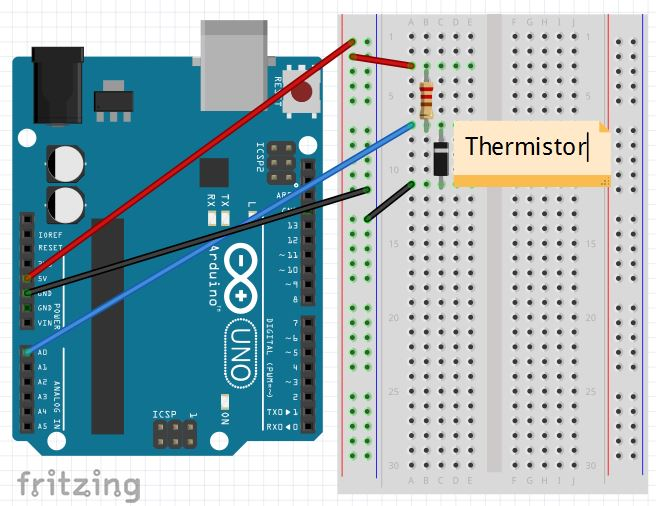
\includegraphics[width=0.5\linewidth]{temperaturefritzing1.jpg}
	\caption{Thermistor in Voltage Divider Configuration using Fritzing}
	\label{temperaturefritzing1}
\end{figure}

The datasheet of the material type F thermistor \cite{thermistor} reveals the following formulae and properties: 

\begin{figure}[H]
	\centering
	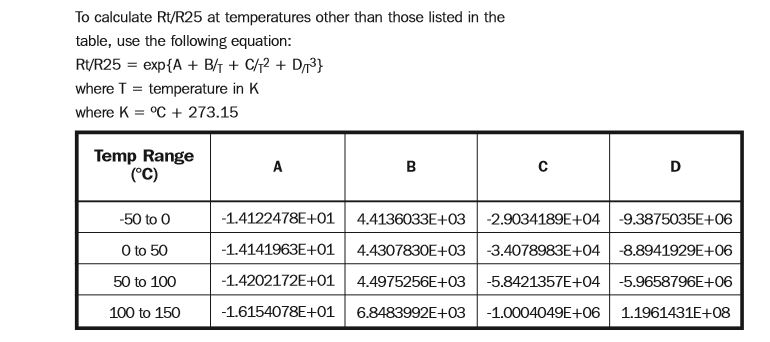
\includegraphics[width=0.8\linewidth]{thermistordatasheet2.jpg}
	\caption{Thermistor Formulae and Properties \cite{thermistor}}
	\label{thermistordatasheet2}
\end{figure}

\begin{figure}[H]
	\centering
	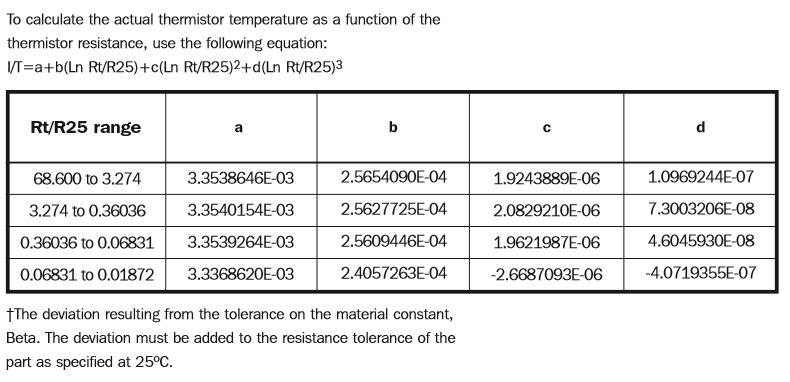
\includegraphics[width=0.8\linewidth]{thermistordatasheet3.jpg}
	\caption{Thermistor Formulae and Properties (cont.) \cite{thermistor}}
	\label{thermistordatasheet3}
\end{figure}

\begin{equation}
	\frac{Rt}{R25} = exp(A+\frac{B}{T}+\frac{C}{T^2}+\frac{D}{T^3}) 
	\label{thermistorresistance1}
\end{equation}

\begin{equation}
	\frac{1}{T} = a+b(ln\frac{Rt}{R25})+c(ln\frac{Rt}{R25})^2+d(ln\frac{Rt}{R25})^3\\
	\label{thermistorresistance2}
\end{equation}

T is the temperature in Kelvin where $K=\degree C+273.15$. 

Choosing an operating temperature range of $0\degree C$ to $50\degree C$, Equation \ref{thermistorresistance1} and \ref{thermistorresistance2} has the following parameters: 

\begin{table}[H]
	\centering
	\caption{Material Type F Thermistor Parameters for $0\degree C$ to $50\degree C$}
	\label{thermistorparameters}
	\begin{tabular}{|l|l|}
		\hline
		A = -1.4141963E+01  & a = 3.3540154E-03 \\ \hline
		B = 4.4307830E+03   & b = 2.5627725E-04 \\ \hline
		C = -3.40789983E+04 & c = 2.0829210E-06 \\ \hline
		D = -8.8941929E+06  & d = 7.3003206E-08 \\ \hline
	\end{tabular}
\end{table}

Therefore, we know that the range of $\frac{Rt}{R25}$ is between 0.36036 to 3.274. $R_{25}$ was chosen to be $10k\Omega$. This circuit was tested with the Arduino code found in Appendix \ref{arduinothermistor}.





It is also known that this material type F thermistor is a negative temperature coefficient (NTC) thermistor, that is, when the temperature rises, there is a decrease in resistance. 

\subsection{Self-Heating - Phase Shift Oscillator}

How does the phase shift oscillator actually work

How does the PSO help in reducing self-heating
Frequency becomes temperature dependent - Voltage not high across the thermistor 

PSO - Bipolar transistor Implementation \cite{psotutorial}

\subsection{Astable Operation of 555 Timer}

Another method of signal condition for the thermistor involves using the 555 Timer in astable operation. 

555 Timer Datasheet. 

\section{Interface}

\subsection{USB}

\subsection{Arduino Uno / Arduino Pro Mini - Analog to Digital Conversion}
\label{arduino}

Arduino Pro Mini 328 - 3.3V/8MHz

\subsubsection{Sensitivity of Arduino Uno} 

1023 bits